%==============================================================================
% CampusLink — Prototype Stage Project Report
% UCS503 Software Engineering Lab, Thapar Institute of Engineering and Technology
%
% Compiles with the TIET report class (https://ctan.org/pkg/tietreport).
% On Overleaf: upload tietreport.cls alongside this file, or the template
% project already contains it. Compiler: pdfLaTeX. Run twice for the ToC and
% cross-references, or just press Recompile twice.
%
% Every diagram is drawn in TikZ, so there are no image files to upload and
% nothing to go missing.
%==============================================================================

\documentclass[twoside,12pt]{tietreport}

\usepackage{tikz}
\usetikzlibrary{arrows.meta,positioning,shapes.geometric,fit,calc,backgrounds,decorations.pathreplacing}
\usepackage{booktabs}
\usepackage{longtable}
\usepackage{array}
\usepackage{enumitem}
\usepackage{xcolor}
\usepackage{listings}
\usepackage{caption}

%------------------------------------------------------------------------------
% Palette. Kept muted so the report prints legibly in greyscale, which is how
% it will most likely be handed in.
%------------------------------------------------------------------------------
\definecolor{tietblue}{HTML}{1F4E79}
\definecolor{tietgrey}{HTML}{5A5A5A}
\definecolor{tietlight}{HTML}{EEF2F7}
\definecolor{tietaccent}{HTML}{B04A35}
\definecolor{tietgreen}{HTML}{2E6B4F}

%------------------------------------------------------------------------------
% Diagram styles, defined once so every figure in the report looks like it
% belongs to the same document.
%------------------------------------------------------------------------------
\tikzset{
  usecase/.style={
    ellipse, draw=tietblue, fill=tietlight, thick,
    minimum width=3.1cm, minimum height=0.95cm,
    align=center, font=\scriptsize, inner sep=1pt
  },
  usecaseplanned/.style={
    usecase, draw=tietgrey, fill=white, dashed
  },
  boundary/.style={
    draw=tietblue, thick, rounded corners=3pt, inner sep=10pt
  },
  class/.style={
    rectangle, draw=tietblue, thick, fill=white,
    align=left, font=\scriptsize, inner sep=4pt, minimum width=3.4cm
  },
  classplanned/.style={class, draw=tietgrey, dashed},
  lifeline/.style={draw=tietgrey, dashed, thick},
  actorbox/.style={
    rectangle, draw=tietblue, thick, fill=tietlight,
    align=center, font=\scriptsize\bfseries, minimum height=0.8cm, inner sep=4pt
  },
  msg/.style={-{Stealth[length=2mm]}, thick, draw=tietblue, font=\scriptsize},
  retmsg/.style={-{Stealth[length=2mm]}, thick, draw=tietgrey, dashed, font=\scriptsize},
  act/.style={
    rectangle, rounded corners=4pt, draw=tietblue, thick, fill=tietlight,
    align=center, font=\scriptsize, minimum width=2.6cm, minimum height=0.8cm
  },
  decision/.style={
    diamond, draw=tietaccent, thick, fill=white, aspect=1.9,
    align=center, font=\scriptsize, inner sep=1pt
  },
  terminal/.style={
    rectangle, rounded corners=10pt, draw=tietgreen, very thick, fill=white,
    align=center, font=\scriptsize\bfseries, minimum width=2.2cm
  },
  flow/.style={-{Stealth[length=2.2mm]}, thick, draw=tietgrey},
  comp/.style={
    rectangle, draw=tietblue, thick, fill=white, align=center,
    font=\scriptsize, minimum width=2.9cm, minimum height=1.0cm
  }
}

% A stick-figure actor, since the use case diagram needs several of them.
\newcommand{\actor}[3]{%
  \begin{scope}[shift={(#1,#2)}]
    \draw[thick,tietblue] (0,0.42) circle (0.16);
    \draw[thick,tietblue] (0,0.26) -- (0,-0.18);
    \draw[thick,tietblue] (-0.22,0.10) -- (0.22,0.10);
    \draw[thick,tietblue] (0,-0.18) -- (-0.18,-0.52);
    \draw[thick,tietblue] (0,-0.18) -- (0.18,-0.52);
    \node[font=\scriptsize\bfseries, align=center, text=tietblue] at (0,-0.85) {#3};
  \end{scope}%
}

\lstset{
  basicstyle=\ttfamily\scriptsize,
  backgroundcolor=\color{tietlight},
  frame=single,
  rulecolor=\color{tietgrey},
  breaklines=true,
  columns=fullflexible,
  keepspaces=true,
  showstringspaces=false,
  captionpos=b,
  xleftmargin=6pt,
  framexleftmargin=6pt
}

%==============================================================================
% Title page
%==============================================================================

\TitlePageHeader{%
  UCS503 Software Engineering Lab%
}

\ProjectTitle{%
  CampusLink%
}

\ProjectSubTitle{%
  A Goal-Matching and Resource-Sharing Platform for College Campuses%
}

\author{%
  \texttt{1024030968} Govind \\
  \texttt{1024030096} Ashish Bajaj \\
  \texttt{ROLLNO3} Teammate Name%
}

\TitlePageSubText{%
  Group: \texttt{GROUP} \quad BE Third Year, Computer Science and Engineering%
}

\AdvisorName{%
  Ms. Anushka%
}

\TitlePageFooterText{{%
    \large Prototype Stage Evaluation \\[0.2cm]
    \bfseries Computer Science and Engineering Department%
  } \\[0.15cm]
  Thapar Institute of Engineering and Technology, Patiala%
}

\begin{document}

\maketitle
\tableofcontents
\listoffigures

%==============================================================================
\chapter{Introduction}
%==============================================================================

\section{Higher-Order Goal}

On a large residential campus, the limiting factor on doing something is rarely
willingness and rarely facilities. It is coordination. A student who wants a gym
partner at six in the morning, a fourth for badminton, someone to split a cab to
the railway station, or last semester's operating systems notes is almost
certainly not alone in wanting it. They simply have no way of finding the other
person before the moment passes.

The broader aim of CampusLink is to make that discovery reliable rather than
accidental, and to put enough structure around the resulting interaction that
meeting a stranger from the same campus feels safe enough to actually do.

\section{Problem Statement}

Everyday coordination on campus currently happens through fragmented informal
channels: batch WhatsApp groups, hostel groups, class groups, and word of mouth.
This produces four concrete problems.

\begin{description}[leftmargin=1.6cm,style=nextline]
  \item[Limited reach] A student's plan reaches only the groups they are already
    in. Compatible people one hostel away never see it. The probability of a
    match is a function of an existing social graph rather than of shared intent.
  \item[No structure for interaction between strangers] A one-to-one plan with
    somebody unknown, particularly a late-night one, needs trust signals that a
    group chat cannot provide. Without them, students self-restrict to people
    they already know, which defeats the purpose.
  \item[Inefficient resource sharing] Notes, past papers and reference material
    circulate as forwarded files with no index, no ownership and no way to ask
    for something specific.
  \item[No accountability] Somebody who repeatedly agrees to a plan and does not
    turn up carries no record of having done so. The cost of an unreliable
    participant falls entirely on the person who was let down.
\end{description}

\section{Proposed Solution}

CampusLink is built around a single loop, deliberately kept small:

\begin{center}
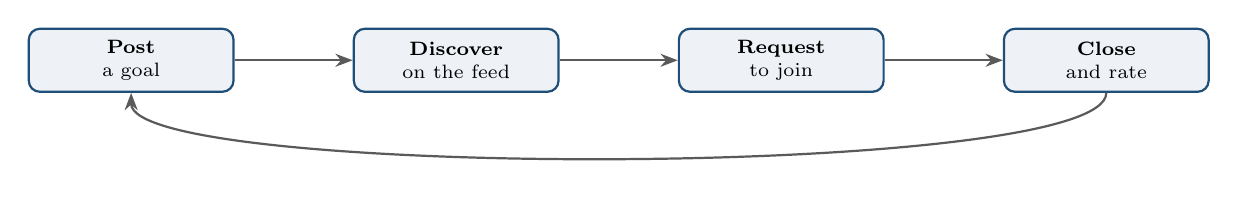
\begin{tikzpicture}[node distance=1.5cm]
  \node[act] (post) {\textbf{Post}\\a goal};
  \node[act, right=of post] (discover) {\textbf{Discover}\\on the feed};
  \node[act, right=of discover] (request) {\textbf{Request}\\to join};
  \node[act, right=of request] (close) {\textbf{Close}\\and rate};
  \draw[flow] (post) -- (discover);
  \draw[flow] (discover) -- (request);
  \draw[flow] (request) -- (close);
  \draw[flow] (close.south) .. controls +(0,-1.1) and +(0,-1.1) .. (post.south);
\end{tikzpicture}
\end{center}

A student posts a \emph{goal} — an activity that needs at least one other person.
The goal appears on a public campus feed. Interested students \emph{request} to
join. The poster accepts or rejects, and once enough people are accepted a
\emph{lobby} forms and the group coordinates the rest in one place. Around that
loop sits a trust and safety layer: verified college identity, reliability
scores, anonymous posting before acceptance, gender-preference restrictions,
report and block controls, and no-show flagging.

\section{Objectives}

\begin{enumerate}[leftmargin=*]
  \item Restrict the platform to verified members of the institute, by requiring
    a \texttt{@thapar.edu} email address and confirming ownership of it through a
    one-time passcode delivered to that inbox.
  \item Let a student post a goal carrying everything another student needs in
    order to decide: category, description, date and time, and how many people
    are still needed.
  \item Present a public feed that is filterable and paginated, and that never
    shows a goal whose time has already passed.
  \item Implement the request and approval state machine that turns a post into a
    committed group.
  \item Enforce every privacy guarantee on the server rather than in the
    interface, so that a promise made to a user cannot be broken by a modified
    client.
  \item Record reliability so that participation history becomes a visible signal.
\end{enumerate}

\section{Scope of This Report}

This is the \textbf{prototype stage} report. It documents a system that runs, and
it is careful to distinguish what has been built from what has been designed but
not yet implemented. Throughout the report, diagrams use \textbf{solid outlines
for implemented elements and dashed outlines for planned ones}, so the state of
the project can be read directly off any figure rather than taken on trust.

Chapter~\ref{ch:requirements} states the requirements and identifies the actors.
Chapter~\ref{ch:design} contains the use case diagram and the supporting UML
models. Chapter~\ref{ch:implementation} describes what has been implemented and
justifies the significant engineering decisions. Chapter~\ref{ch:testing}
covers verification. Chapter~\ref{ch:status} reports honestly on current status,
including what does not yet work and which parts of the original proposal were
deliberately cut.

%==============================================================================
\chapter{Requirements Specification}
\label{ch:requirements}
%==============================================================================

\section{Actors}

Identifying the actors correctly matters more than it first appears, because two
of them are not people, and forgetting them produces a design that cannot explain
how a passcode arrives or how an expired goal leaves the feed.

\begin{longtable}{@{}p{3.4cm}p{2.2cm}p{7.4cm}@{}}
\toprule
\textbf{Actor} & \textbf{Type} & \textbf{Description} \\
\midrule
\endhead
Student &
Primary, human &
Any verified member of the institute. The same person is a \emph{poster} on
goals they create and a \emph{requester} on goals they join, so these are roles
rather than separate actors. Modelling them as two actors would wrongly suggest
two accounts. \\
\addlinespace
Moderator &
Primary, human &
A student with an elevated role who reviews reports and can unmask an anonymous
poster when a report is upheld. Every such action is audit-logged. \\
\addlinespace
Email Service &
Secondary, external &
The SMTP provider that delivers verification passcodes. It is an actor because
the registration use case cannot complete without a response from it, and
because its failure is a case the system must handle rather than ignore. \\
\addlinespace
Scheduler &
Secondary, system &
Time itself, as an actor. Goals expire and lobbies close without any human
initiating it. Modelling this explicitly is what forces the design to answer
what happens to a goal nobody joined. \\
\bottomrule
\end{longtable}

\section{Functional Requirements}

\begin{longtable}{@{}p{1.4cm}p{8.2cm}p{3.2cm}@{}}
\toprule
\textbf{ID} & \textbf{Requirement} & \textbf{Status} \\
\midrule
\endhead
FR-1 & The system shall accept registration only from addresses in the
        \texttt{thapar.edu} domain. & Implemented \\
FR-2 & The system shall confirm ownership of the address by emailing a six-digit
        passcode that expires in ten minutes. & Implemented \\
FR-3 & The system shall limit passcode attempts and invalidate a passcode once
        used. & Implemented \\
FR-4 & The system shall authenticate returning students and issue a session
        token. & Implemented \\
FR-5 & A student shall be able to maintain a profile: name, branch, year of
        study, gender, interests and a photograph. & Implemented \\
FR-6 & A student shall be able to post a goal with category, title, description,
        optional date and time, and headcount. & Implemented \\
FR-7 & A student shall be able to post a goal anonymously, with identity revealed
        only after acceptance. & Implemented \\
FR-8 & A student shall be able to restrict who may request to join by gender
        preference. & Implemented \\
FR-9 & The system shall present a public feed, filterable by category and date,
        paginated, excluding expired goals. & Implemented \\
FR-10 & A poster shall be able to cancel their own goal. & Implemented \\
FR-11 & A student shall be able to request to join a goal. & Planned \\
FR-12 & A poster shall be able to accept or reject a request, or enable automatic
        acceptance until the headcount is met. & Planned \\
FR-13 & The system shall form a lobby once the headcount is met. & Planned \\
FR-14 & Lobby members shall be able to exchange messages in real time. & Planned \\
FR-15 & A participant shall be able to rate others and flag a no-show after
        completion. & Planned \\
FR-16 & A student shall be able to report or block another student. & Planned \\
FR-17 & A moderator shall be able to review reports and unmask an anonymous
        poster, with the action audit-logged. & Planned \\
\bottomrule
\end{longtable}

\section{Non-Functional Requirements}

\begin{longtable}{@{}p{1.6cm}p{3.0cm}p{8.2cm}@{}}
\toprule
\textbf{ID} & \textbf{Attribute} & \textbf{Requirement} \\
\midrule
\endhead
NFR-1 & Security &
Passwords shall never be stored in recoverable form. Passcodes shall be stored
only as hashes, so that a leaked database does not permit impersonation. \\
\addlinespace
NFR-2 & Privacy &
Anonymity shall be enforced by omitting identity from the server's response, not
by hiding it in the interface. A client cannot reveal what it was never sent. \\
\addlinespace
NFR-3 & Integrity &
A student shall not be able to modify their own role, verification state or
reliability score through any endpoint. \\
\addlinespace
NFR-4 & Performance &
The feed shall be paginated and served from indexed queries, and shall not
degrade as the number of goals grows. \\
\addlinespace
NFR-5 & Portability &
The schema shall run unchanged on both the development database and the
production database, so that deployment is a configuration change. \\
\addlinespace
NFR-6 & Usability &
The interface shall be usable on a phone, since the proposal expects most use to
occur there. \\
\addlinespace
NFR-7 & Maintainability &
Validation rules shall have exactly one definition, shared by client and server,
so the two cannot disagree. \\
\bottomrule
\end{longtable}

%==============================================================================
\chapter{System Design}
\label{ch:design}
%==============================================================================

\section{Use Case Diagram}

Figure~\ref{fig:usecase} is the use case diagram for CampusLink. Solid ellipses
are use cases that are implemented and demonstrable; dashed ellipses are
specified and designed but not yet built.

\begin{figure}[p]
\centering
\resizebox{!}{0.86\textheight}{%
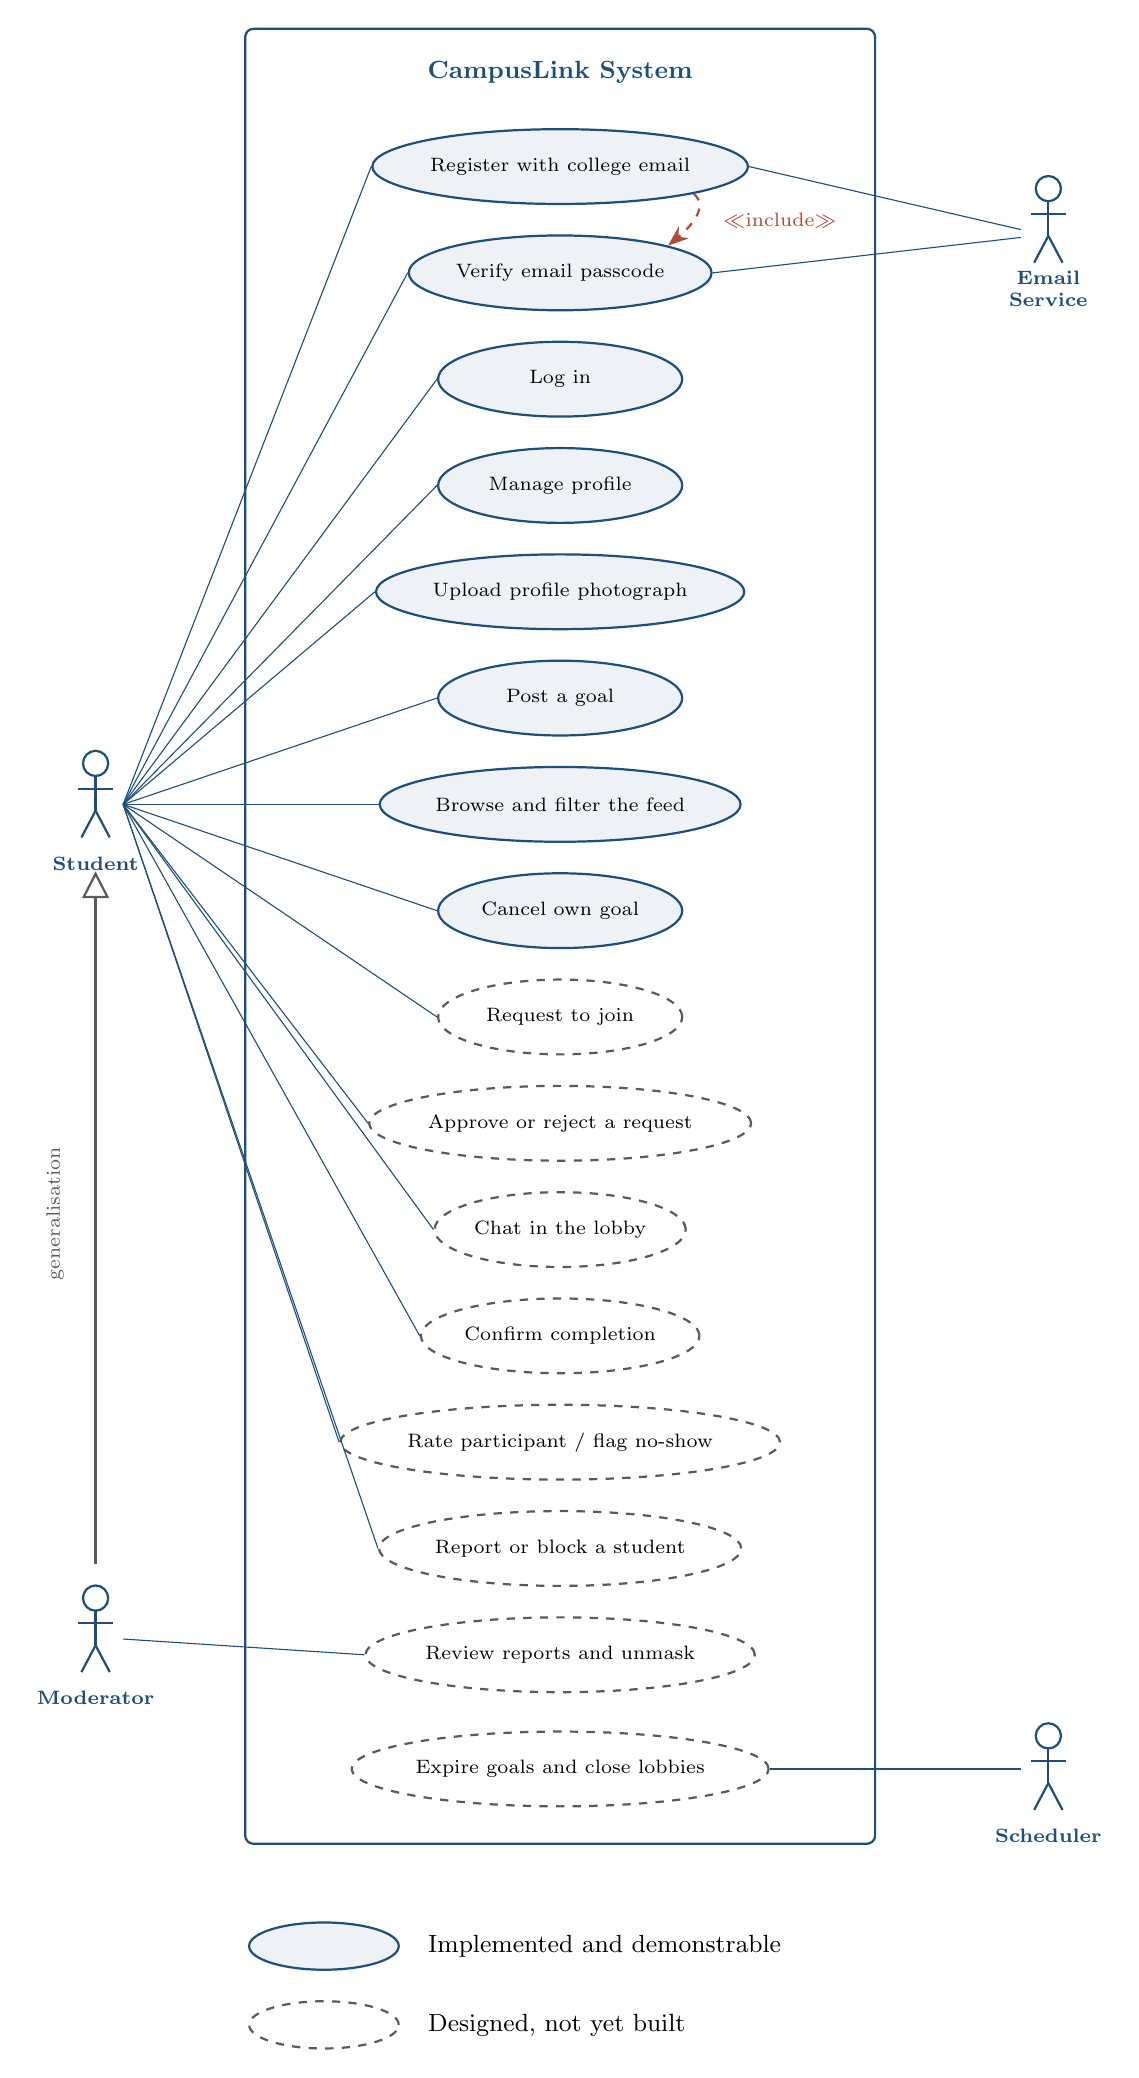
\begin{tikzpicture}

  % ---- System boundary ----------------------------------------------------
  \draw[boundary] (3.4,1.15) rectangle (11.4,-21.9);
  \node[font=\small\bfseries, text=tietblue] at (7.4,0.6) {CampusLink System};

  % ---- Use cases, one column so that no association crosses an ellipse -----
  \node[usecase] (uc1)  at (7.4,-0.6)   {Register with college email};
  \node[usecase] (uc2)  at (7.4,-1.95)  {Verify email passcode};
  \node[usecase] (uc3)  at (7.4,-3.30)  {Log in};
  \node[usecase] (uc4)  at (7.4,-4.65)  {Manage profile};
  \node[usecase] (uc5)  at (7.4,-6.00)  {Upload profile photograph};
  \node[usecase] (uc6)  at (7.4,-7.35)  {Post a goal};
  \node[usecase] (uc7)  at (7.4,-8.70)  {Browse and filter the feed};
  \node[usecase] (uc8)  at (7.4,-10.05) {Cancel own goal};

  \node[usecaseplanned] (uc9)  at (7.4,-11.40) {Request to join};
  \node[usecaseplanned] (uc10) at (7.4,-12.75) {Approve or reject a request};
  \node[usecaseplanned] (uc11) at (7.4,-14.10) {Chat in the lobby};
  \node[usecaseplanned] (uc12) at (7.4,-15.45) {Confirm completion};
  \node[usecaseplanned] (uc13) at (7.4,-16.80) {Rate participant / flag no-show};
  \node[usecaseplanned] (uc14) at (7.4,-18.15) {Report or block a student};
  \node[usecaseplanned] (uc15) at (7.4,-19.50) {Review reports and unmask};
  \node[usecaseplanned] (uc16) at (7.4,-20.95) {Expire goals and close lobbies};

  % ---- Actors --------------------------------------------------------------
  \actor{1.5}{-8.6}{Student}
  \actor{1.5}{-19.2}{Moderator}
  \actor{13.6}{-1.3}{Email\\Service}
  \actor{13.6}{-20.95}{Scheduler}

  % ---- Student associations ------------------------------------------------
  \foreach \t in {uc1,uc2,uc3,uc4,uc5,uc6,uc7,uc8,uc9,uc10,uc11,uc12,uc13,uc14}
    \draw[tietblue, thin] (1.85,-8.7) -- (\t.west);

  % ---- Moderator -----------------------------------------------------------
  \draw[tietblue, thin] (1.85,-19.3) -- (uc15.west);

  % A moderator holds a normal student account with an elevated role, so every
  % student use case is inherited rather than repeated here.
  \draw[-{Triangle[open,length=3.4mm,width=3.4mm]}, thick, tietgrey]
    (1.5,-18.35) -- (1.5,-9.55);
  \node[font=\scriptsize, text=tietgrey, rotate=90, anchor=south] at (1.22,-13.9)
    {generalisation};

  % ---- Secondary actors ----------------------------------------------------
  \draw[tietblue, thin] (uc1.east) -- (13.25,-1.4);
  \draw[tietblue, thin] (uc2.east) -- (13.25,-1.5);
  \draw[tietblue, thin] (uc16.east) -- (13.25,-20.95);

  % ---- Include, routed to the right so it clears the association fan -------
  \draw[-{Stealth[length=2.6mm]}, dashed, thick, tietaccent]
    (uc1.south east) to[out=-40,in=40] (uc2.north east);
  \node[font=\scriptsize, text=tietaccent, anchor=west] at (9.35,-1.28)
    {$\ll$include$\gg$};

  % ---- Legend --------------------------------------------------------------
  \node[usecase, minimum width=1.9cm, minimum height=0.6cm] at (4.4,-23.2) {};
  \node[anchor=west, font=\small] at (5.6,-23.2) {Implemented and demonstrable};
  \node[usecaseplanned, minimum width=1.9cm, minimum height=0.6cm] at (4.4,-24.2) {};
  \node[anchor=west, font=\small] at (5.6,-24.2) {Designed, not yet built};

\end{tikzpicture}%
}
\caption[Use case diagram for CampusLink]{Use case diagram. The Student and
Moderator are human actors; the Email Service and the Scheduler are secondary
actors, without which registration and expiry cannot be explained.}
\label{fig:usecase}
\end{figure}

\subsection{Justification of the Relationships}

Anticipating the questions likely to be asked about this diagram:

\begin{description}[leftmargin=0.8cm,style=nextline]
  \item[Why is ``poster'' not an actor?]
    Because it is a role, not a person. The same student posts one goal and
    requests to join another within the same session. Drawing Poster and
    Requester as separate actors would imply two accounts and two identities,
    which is precisely what the design does not do.

  \item[Why is Moderator generalised from Student?]
    A moderator holds a normal student account with an elevated \texttt{role}
    field. They register, log in and post goals exactly as anybody else does.
    Generalisation states that they inherit every student use case and add one,
    which is a truthful description of the implementation and avoids repeating
    eight associations.

  \item[Why is the Email Service an actor at all?]
    Because registration cannot complete without it. If the passcode is not
    delivered, the use case fails, and the system must react — in the
    implementation, the passcode row is deleted and an error is returned, so
    nobody is left waiting for a code that was never sent. An external system
    that a use case depends on and whose failure changes the outcome is an actor.

  \item[Why is the Scheduler an actor?]
    Goals expire without anybody pressing anything. Modelling time as an actor
    is what forces the design to answer the question ``what happens to a goal
    nobody joined?'' rather than leaving it unanswered.

  \item[Why $\ll$include$\gg$ from Register to Verify?]
    Registration is not complete until the passcode is confirmed; the included
    use case always executes as part of the base one. It is not
    $\ll$extend$\gg$, because verification is not optional.
\end{description}

\subsection{Include and Extend Around the Core Use Cases}

Figure~\ref{fig:extend} isolates the two use cases at the centre of the product
so that the optional and mandatory sub-behaviours are legible.

\begin{figure}[htbp]
\centering
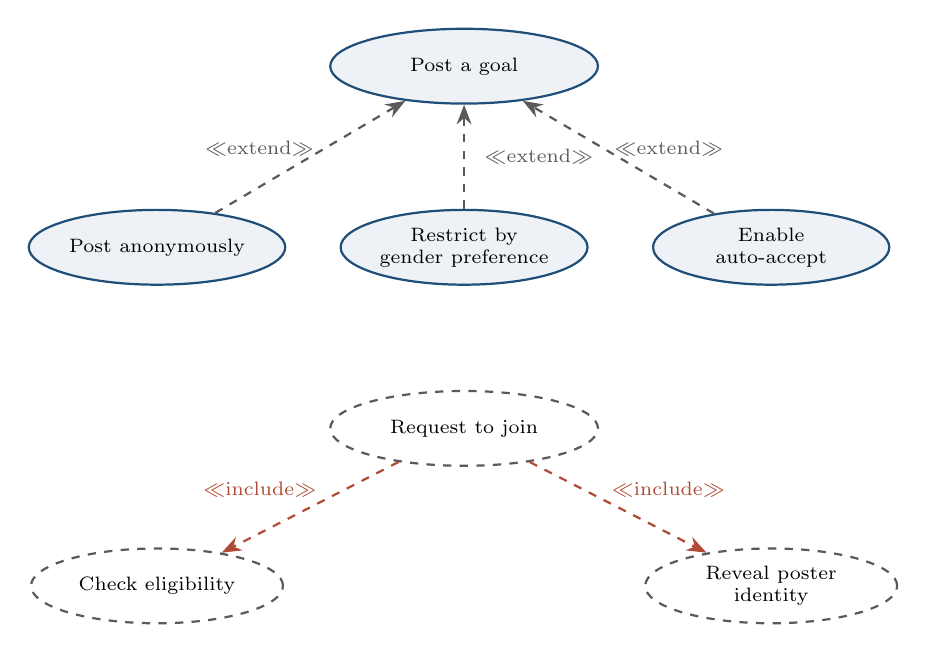
\begin{tikzpicture}

  \node[usecase, minimum width=3.4cm] (post) at (0,0) {Post a goal};
  \node[usecase, minimum width=3.0cm] (anon) at (-3.9,-2.3) {Post anonymously};
  \node[usecase, minimum width=3.0cm] (gender) at (0,-2.3) {Restrict by\\gender preference};
  \node[usecase, minimum width=3.0cm] (auto) at (3.9,-2.3) {Enable\\auto-accept};

  \foreach \t in {anon,gender,auto}
    \draw[-{Stealth[length=2.5mm]}, dashed, thick, tietgrey] (\t) -- (post);
  \node[font=\scriptsize, text=tietgrey] at (-2.6,-1.05) {$\ll$extend$\gg$};
  \node[font=\scriptsize, text=tietgrey] at (0.95,-1.15) {$\ll$extend$\gg$};
  \node[font=\scriptsize, text=tietgrey] at (2.6,-1.05) {$\ll$extend$\gg$};

  \node[usecaseplanned, minimum width=3.4cm] (req) at (0,-4.6) {Request to join};
  \node[usecaseplanned, minimum width=3.2cm] (check) at (-3.9,-6.6) {Check eligibility};
  \node[usecaseplanned, minimum width=3.2cm] (reveal) at (3.9,-6.6) {Reveal poster\\identity};

  \draw[-{Stealth[length=2.5mm]}, dashed, thick, tietaccent] (req) -- (check)
    node[midway,above left,font=\scriptsize,text=tietaccent,xshift=6pt] {$\ll$include$\gg$};
  \draw[-{Stealth[length=2.5mm]}, dashed, thick, tietaccent] (req) -- (reveal)
    node[midway,above right,font=\scriptsize,text=tietaccent,xshift=-6pt] {$\ll$include$\gg$};

\end{tikzpicture}
\caption[Include and extend relationships]{Anonymity, gender restriction and
auto-accept are $\ll$extend$\gg$: a goal is perfectly valid without any of them.
Eligibility checking and identity reveal are $\ll$include$\gg$: they always run
as part of a join request.}
\label{fig:extend}
\end{figure}

\section{Class Diagram}

Figure~\ref{fig:class} is the class diagram. It corresponds directly to the
database schema — every implemented class is a table, and the attribute lists are
the actual columns rather than an idealised version of them.

\begin{figure}[htbp]
\centering
\resizebox{0.98\textwidth}{!}{%
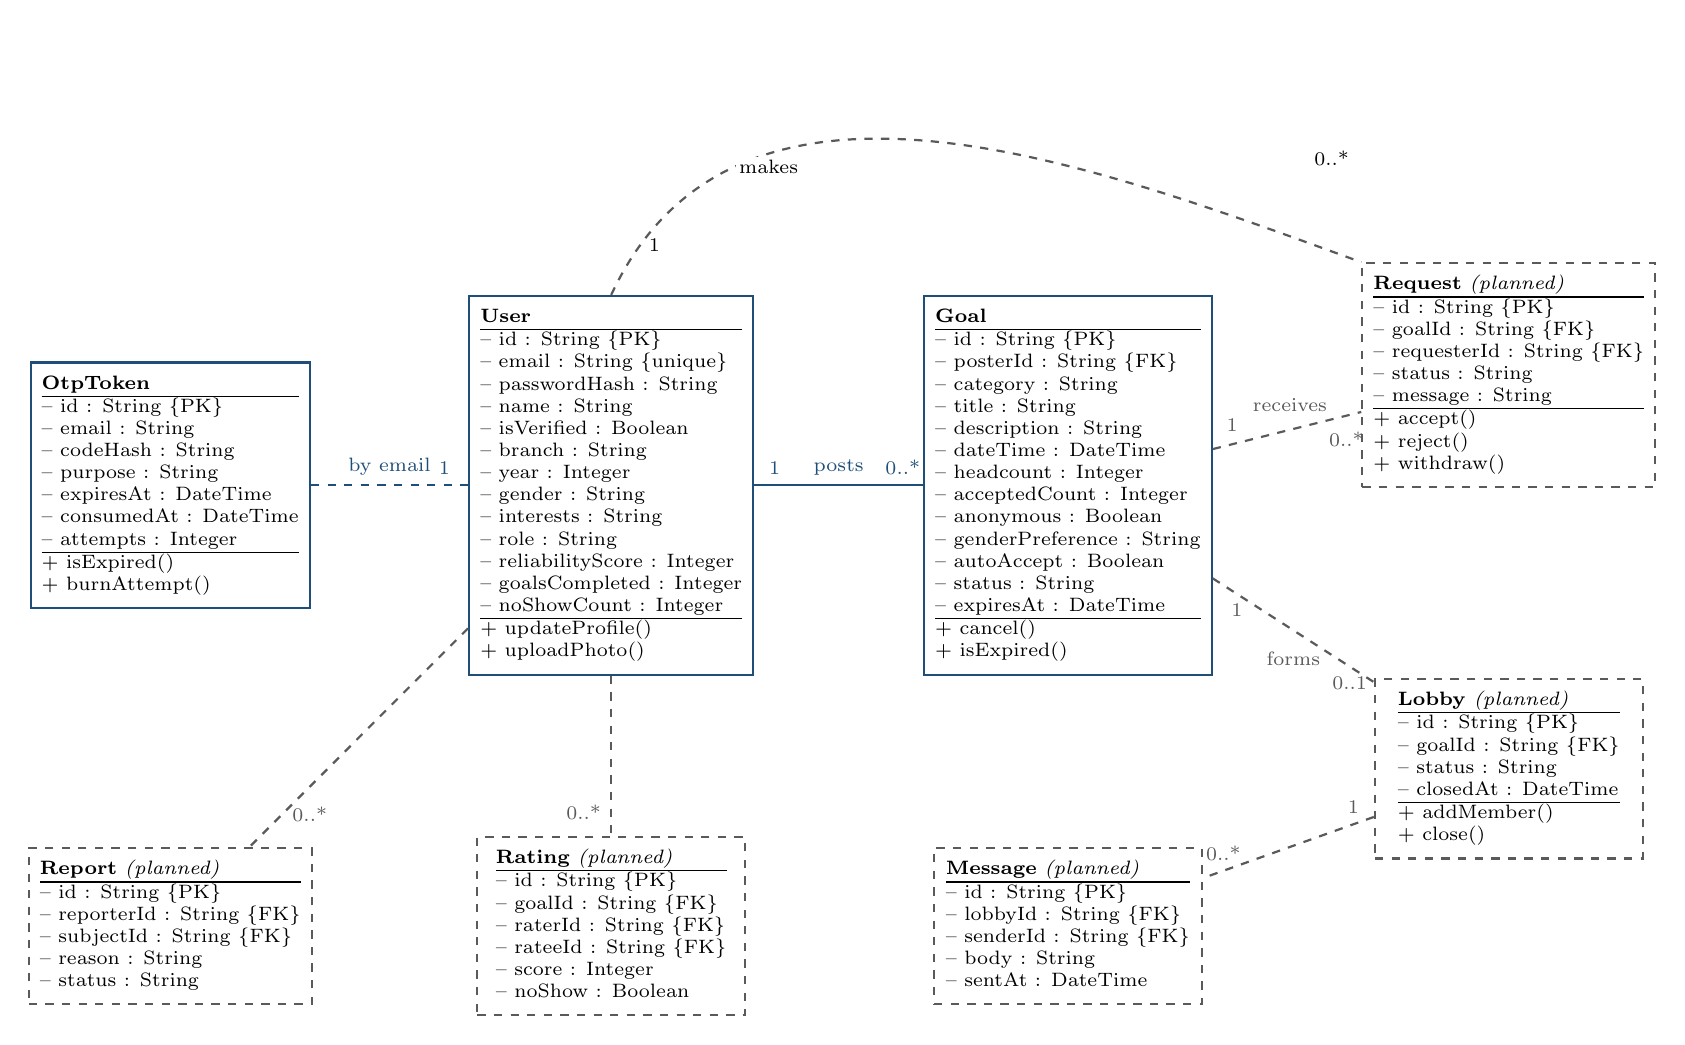
\begin{tikzpicture}

  \node[class] (user) at (0,0) {%
    \begin{tabular}{@{}l@{}}
      \textbf{User}\\\hline
      -- id : String \{PK\}\\
      -- email : String \{unique\}\\
      -- passwordHash : String\\
      -- name : String\\
      -- isVerified : Boolean\\
      -- branch : String\\
      -- year : Integer\\
      -- gender : String\\
      -- interests : String\\
      -- role : String\\
      -- reliabilityScore : Integer\\
      -- goalsCompleted : Integer\\
      -- noShowCount : Integer\\\hline
      + updateProfile()\\
      + uploadPhoto()\\
    \end{tabular}};

  \node[class] (otp) at (-5.6,0) {%
    \begin{tabular}{@{}l@{}}
      \textbf{OtpToken}\\\hline
      -- id : String \{PK\}\\
      -- email : String\\
      -- codeHash : String\\
      -- purpose : String\\
      -- expiresAt : DateTime\\
      -- consumedAt : DateTime\\
      -- attempts : Integer\\\hline
      + isExpired()\\
      + burnAttempt()\\
    \end{tabular}};

  \node[class] (goal) at (5.8,0) {%
    \begin{tabular}{@{}l@{}}
      \textbf{Goal}\\\hline
      -- id : String \{PK\}\\
      -- posterId : String \{FK\}\\
      -- category : String\\
      -- title : String\\
      -- description : String\\
      -- dateTime : DateTime\\
      -- headcount : Integer\\
      -- acceptedCount : Integer\\
      -- anonymous : Boolean\\
      -- genderPreference : String\\
      -- autoAccept : Boolean\\
      -- status : String\\
      -- expiresAt : DateTime\\\hline
      + cancel()\\
      + isExpired()\\
    \end{tabular}};

  \node[classplanned] (request) at (11.4,1.4) {%
    \begin{tabular}{@{}l@{}}
      \textbf{Request} \textit{(planned)}\\\hline
      -- id : String \{PK\}\\
      -- goalId : String \{FK\}\\
      -- requesterId : String \{FK\}\\
      -- status : String\\
      -- message : String\\\hline
      + accept()\\
      + reject()\\
      + withdraw()\\
    \end{tabular}};

  \node[classplanned] (lobby) at (11.4,-3.6) {%
    \begin{tabular}{@{}l@{}}
      \textbf{Lobby} \textit{(planned)}\\\hline
      -- id : String \{PK\}\\
      -- goalId : String \{FK\}\\
      -- status : String\\
      -- closedAt : DateTime\\\hline
      + addMember()\\
      + close()\\
    \end{tabular}};

  \node[classplanned] (message) at (5.8,-5.6) {%
    \begin{tabular}{@{}l@{}}
      \textbf{Message} \textit{(planned)}\\\hline
      -- id : String \{PK\}\\
      -- lobbyId : String \{FK\}\\
      -- senderId : String \{FK\}\\
      -- body : String\\
      -- sentAt : DateTime\\
    \end{tabular}};

  \node[classplanned] (rating) at (0,-5.6) {%
    \begin{tabular}{@{}l@{}}
      \textbf{Rating} \textit{(planned)}\\\hline
      -- id : String \{PK\}\\
      -- goalId : String \{FK\}\\
      -- raterId : String \{FK\}\\
      -- rateeId : String \{FK\}\\
      -- score : Integer\\
      -- noShow : Boolean\\
    \end{tabular}};

  \node[classplanned] (report) at (-5.6,-5.6) {%
    \begin{tabular}{@{}l@{}}
      \textbf{Report} \textit{(planned)}\\\hline
      -- id : String \{PK\}\\
      -- reporterId : String \{FK\}\\
      -- subjectId : String \{FK\}\\
      -- reason : String\\
      -- status : String\\
    \end{tabular}};

  % ---- Associations --------------------------------------------------------
  \draw[thick,tietblue] (user) -- (goal)
    node[pos=0.12,above,font=\scriptsize] {1}
    node[pos=0.88,above,font=\scriptsize] {0..*}
    node[midway,above,font=\scriptsize] {posts};

  \draw[thick,tietgrey,dashed] (goal) -- (request)
    node[pos=0.13,above,font=\scriptsize,yshift=1pt] {1}
    node[pos=0.90,below,font=\scriptsize,yshift=-2pt] {0..*}
    node[pos=0.52,above,font=\scriptsize,yshift=3pt] {receives};

  % Routed over the top of the diagram; the label is placed at an explicit
  % coordinate near the apex rather than by pos=, which landed it inside the box.
  \draw[thick,tietgrey,dashed] (user.north) to[out=65,in=160] (request.north west);
  \node[font=\scriptsize, fill=white, inner sep=1pt] at (2.0,4.05) {makes};
  \node[font=\scriptsize] at (0.55,3.05) {1};
  \node[font=\scriptsize] at (9.15,4.15) {0..*};

  \draw[thick,tietgrey,dashed] (goal) -- (lobby)
    node[pos=0.15,below,font=\scriptsize] {1}
    node[pos=0.85,below,font=\scriptsize] {0..1}
    node[midway,below,font=\scriptsize,yshift=-4pt] {forms};

  \draw[thick,tietgrey,dashed] (lobby) -- (message)
    node[pos=0.12,above,font=\scriptsize] {1}
    node[pos=0.88,above,font=\scriptsize] {0..*};

  \draw[thick,tietgrey,dashed] (user) -- (rating)
    node[pos=0.85,left,font=\scriptsize] {0..*};

  \draw[thick,tietgrey,dashed] (user) -- (report)
    node[pos=0.85,right,font=\scriptsize] {0..*};

  % OtpToken is associated by email, not by a foreign key: a passcode is issued
  % before the account is usable, so it cannot point at a verified User row.
  \draw[thick,tietblue,dashed] (otp) -- (user)
    node[midway,above,font=\scriptsize] {by email}
    node[pos=0.85,above,font=\scriptsize] {1};

\end{tikzpicture}%
}
\caption[Class diagram]{Class diagram. Solid classes exist in the database
today; dashed classes are designed and will be added in the steps named in
Chapter~\ref{ch:status}.}
\label{fig:class}
\end{figure}

\subsection{Design Decisions Visible in the Class Diagram}

\begin{description}[leftmargin=0.8cm,style=nextline]
  \item[\texttt{acceptedCount} is denormalised on \texttt{Goal}.]
    Every card on the feed renders ``2 of 3 joined''. Counting accepted requests
    per card would issue one query per row of the feed. Storing the count and
    updating it on the two events that change it trades a small consistency
    obligation for the elimination of an N+1 query.

  \item[\texttt{OtpToken} associates by email, not by foreign key.]
    A passcode is issued during registration, before there is a usable account.
    A foreign key to \texttt{User} would either require the row to exist first or
    fail. Associating by address also lets the same mechanism serve password
    reset later.

  \item[Enumerated attributes are typed \texttt{String}.]
    The development database does not support native enumerated types. Rather
    than maintain two schemas, every enumerated column is a string whose
    permitted values are defined once in the shared validation layer and enforced
    at the API boundary. This is what satisfies NFR-5.

  \item[\texttt{Rating} references the goal as well as both students.]
    Without the goal, the same pair could rate each other repeatedly and inflate
    a reliability score. Anchoring the rating to the completed goal makes ``one
    rating per participant per goal'' expressible as a uniqueness constraint.
\end{description}

\section{Sequence Diagrams}

\subsection{Registration and Email Verification}

Figure~\ref{fig:seq-otp} traces the registration use case. It is the sequence
worth showing in full because it is the only one that depends on an external
actor, and because the failure path is as important as the success path.

\begin{figure}[htbp]
\centering
\resizebox{0.95\textwidth}{!}{%
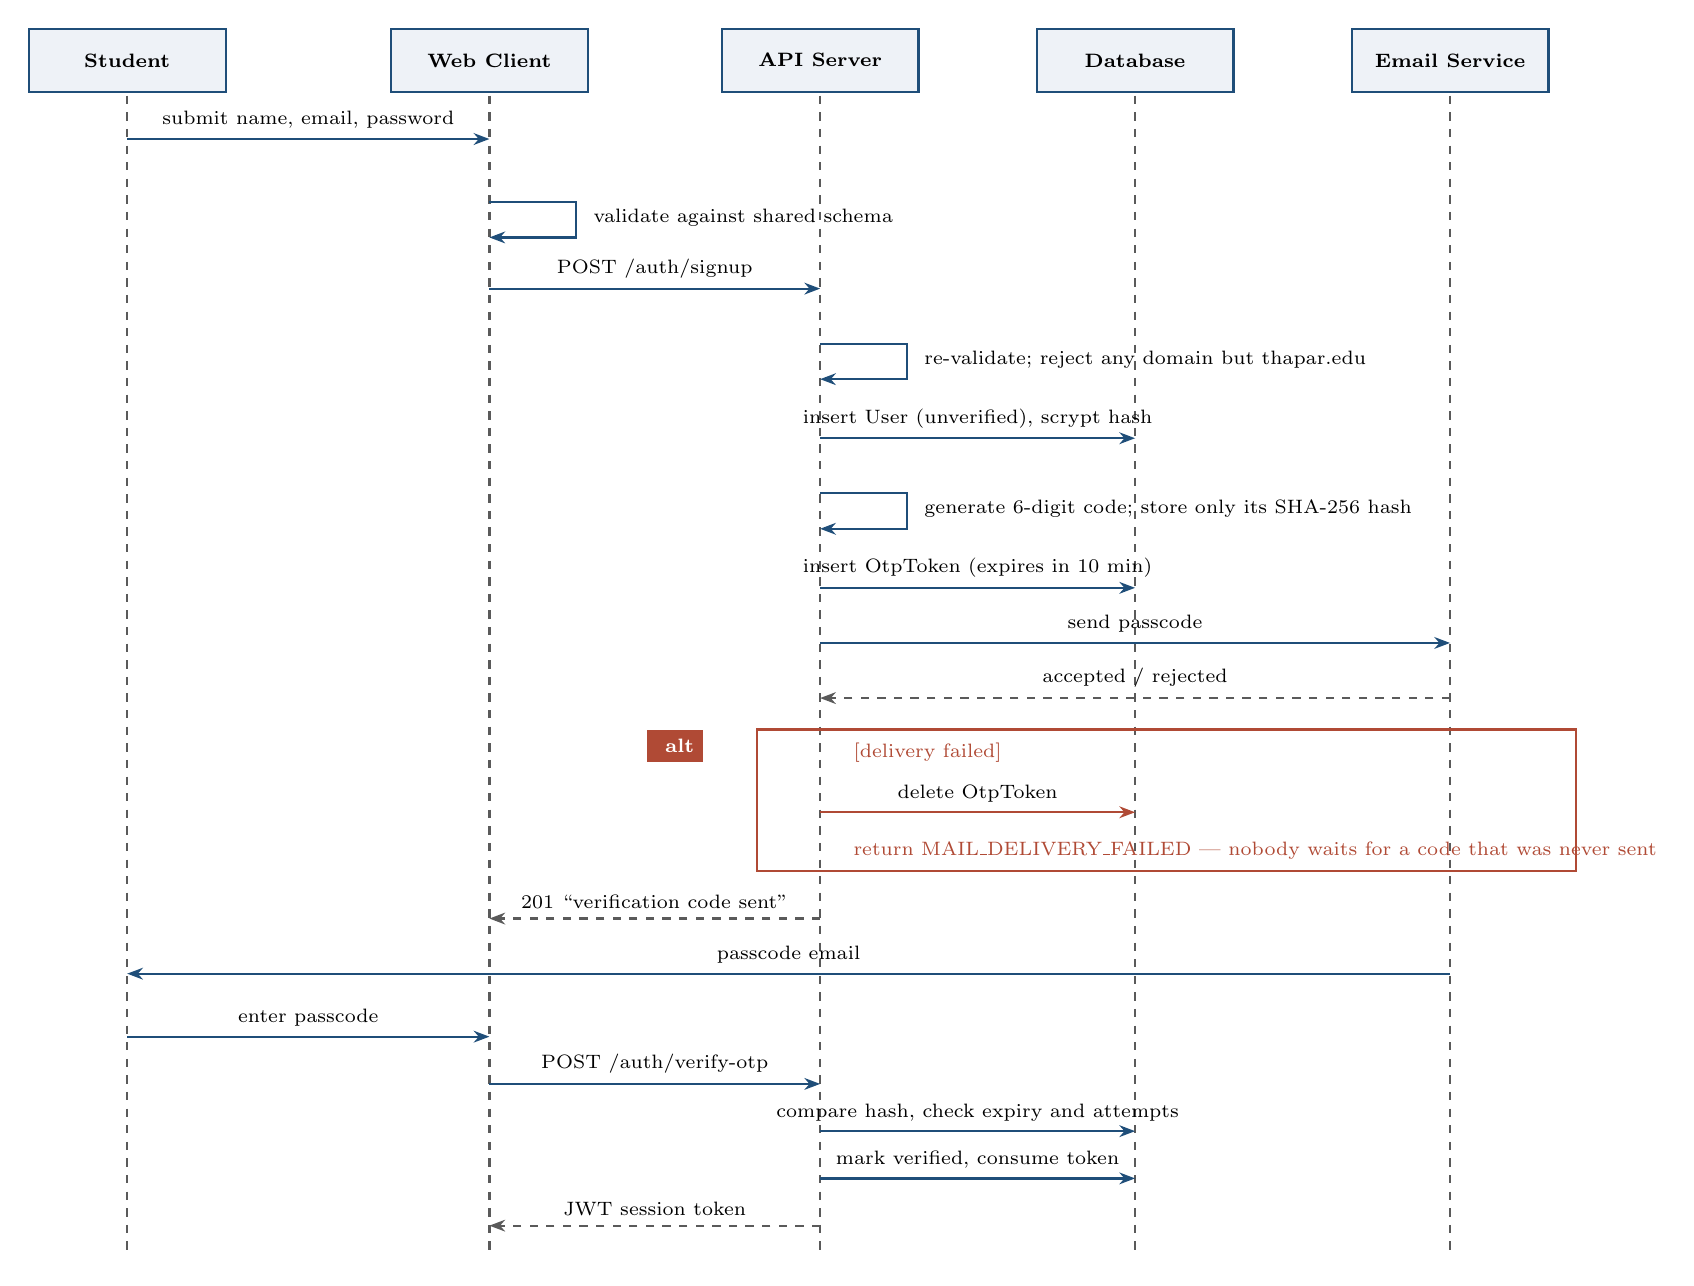
\begin{tikzpicture}[font=\scriptsize]

  % ---- Lifelines -----------------------------------------------------------
  \foreach \x/\name in {0/{Student}, 4.6/{Web Client}, 8.8/{API Server},
                        12.8/{Database}, 16.8/{Email Service}} {
    \node[actorbox, minimum width=2.5cm] at (\x,0) {\name};
    \draw[lifeline] (\x,-0.45) -- (\x,-15.2);
  }

  % ---- Messages ------------------------------------------------------------
  \draw[msg] (0,-1.0) -- node[above]{submit name, email, password} (4.6,-1.0);
  \draw[msg] (4.6,-1.8) -- ++(1.1,0) -- ++(0,-0.45) -- ++(-1.1,0);
  \node[right, font=\scriptsize] at (5.8,-2.0) {validate against shared schema};

  \draw[msg] (4.6,-2.9) -- node[above]{POST /auth/signup} (8.8,-2.9);
  \draw[msg] (8.8,-3.6) -- ++(1.1,0) -- ++(0,-0.45) -- ++(-1.1,0);
  \node[right, font=\scriptsize] at (10.0,-3.8) {re-validate; reject any domain but thapar.edu};

  \draw[msg] (8.8,-4.8) -- node[above]{insert User (unverified), scrypt hash} (12.8,-4.8);
  \draw[msg] (8.8,-5.5) -- ++(1.1,0) -- ++(0,-0.45) -- ++(-1.1,0);
  \node[right, font=\scriptsize] at (10.0,-5.7) {generate 6-digit code; store only its SHA-256 hash};

  \draw[msg] (8.8,-6.7) -- node[above]{insert OtpToken (expires in 10 min)} (12.8,-6.7);
  \draw[msg] (8.8,-7.4) -- node[above]{send passcode} (16.8,-7.4);
  \draw[retmsg] (16.8,-8.1) -- node[above]{accepted / rejected} (8.8,-8.1);

  % ---- Failure fragment ----------------------------------------------------
  \draw[draw=tietaccent, thick] (8.0,-8.5) rectangle (18.4,-10.3);
  \node[fill=tietaccent, text=white, font=\scriptsize\bfseries, anchor=north west]
    at (6.6,-8.5) {\ alt\ };
  \node[anchor=north west, font=\scriptsize, text=tietaccent] at (9.1,-8.55)
    {[delivery failed]};
  \draw[msg, draw=tietaccent] (8.8,-9.55) -- node[above]{delete OtpToken} (12.8,-9.55);
  \node[anchor=north west, font=\scriptsize, text=tietaccent] at (9.1,-9.8)
    {return MAIL\_DELIVERY\_FAILED — nobody waits for a code that was never sent};

  \draw[retmsg] (8.8,-10.9) -- node[above]{201 ``verification code sent''} (4.6,-10.9);
  \draw[msg] (16.8,-11.6) -- node[above]{passcode email} (0,-11.6);

  \draw[msg] (0,-12.4) -- node[above]{enter passcode} (4.6,-12.4);
  \draw[msg] (4.6,-13.0) -- node[above]{POST /auth/verify-otp} (8.8,-13.0);
  \draw[msg] (8.8,-13.6) -- node[above]{compare hash, check expiry and attempts} (12.8,-13.6);
  \draw[msg] (8.8,-14.2) -- node[above]{mark verified, consume token} (12.8,-14.2);
  \draw[retmsg] (8.8,-14.8) -- node[above]{JWT session token} (4.6,-14.8);

\end{tikzpicture}%
}
\caption[Sequence diagram: registration and email verification]{Registration and
email verification. Only the hash of the passcode is stored, so a leaked database
does not allow anybody to verify as somebody else.}
\label{fig:seq-otp}
\end{figure}

\subsection{Anonymous Posting and Feed Retrieval}

Figure~\ref{fig:seq-anon} shows where anonymity is actually enforced. This is the
sequence that demonstrates NFR-2, and the reason the serialiser is drawn as its
own participant rather than folded into the API.

\begin{figure}[htbp]
\centering
\resizebox{0.95\textwidth}{!}{%
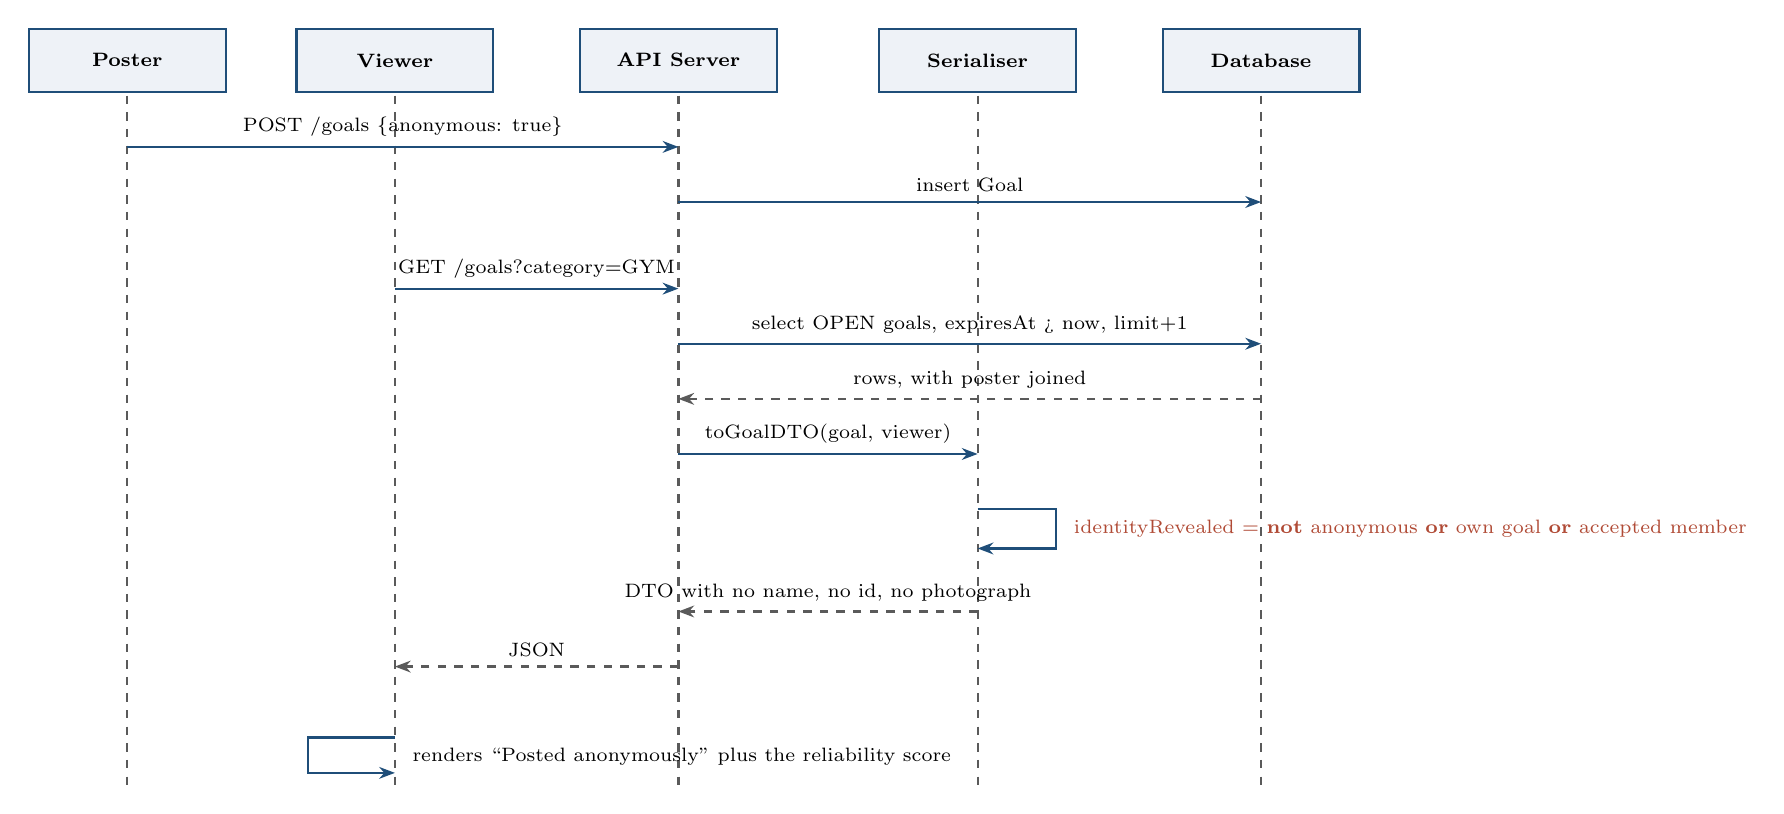
\begin{tikzpicture}[font=\scriptsize]

  \foreach \x/\name in {0/{Poster}, 3.4/{Viewer}, 7.0/{API Server},
                        10.8/{Serialiser}, 14.4/{Database}} {
    \node[actorbox, minimum width=2.5cm] at (\x,0) {\name};
    \draw[lifeline] (\x,-0.45) -- (\x,-9.2);
  }

  \draw[msg] (0,-1.1) -- node[above]{POST /goals \{anonymous: true\}} (7.0,-1.1);
  \draw[msg] (7.0,-1.8) -- node[above]{insert Goal} (14.4,-1.8);

  \draw[msg] (3.4,-2.9) -- node[above]{GET /goals?category=GYM} (7.0,-2.9);
  \draw[msg] (7.0,-3.6) -- node[above]{select OPEN goals, expiresAt > now, limit+1} (14.4,-3.6);
  \draw[retmsg] (14.4,-4.3) -- node[above]{rows, with poster joined} (7.0,-4.3);

  \draw[msg] (7.0,-5.0) -- node[above]{toGoalDTO(goal, viewer)} (10.8,-5.0);
  \draw[msg] (10.8,-5.7) -- ++(1.0,0) -- ++(0,-0.5) -- ++(-1.0,0);
  \node[right, font=\scriptsize, text=tietaccent] at (11.9,-5.95)
    {identityRevealed = \textbf{not} anonymous \textbf{or} own goal \textbf{or} accepted member};

  \draw[retmsg] (10.8,-7.0) -- node[above]{DTO with no name, no id, no photograph} (7.0,-7.0);
  \draw[retmsg] (7.0,-7.7) -- node[above]{JSON} (3.4,-7.7);
  \draw[msg] (3.4,-8.6) -- ++(-1.1,0) -- ++(0,-0.45) -- ++(1.1,0);
  \node[right, font=\scriptsize] at (3.5,-8.85)
    {renders ``Posted anonymously'' plus the reliability score};

\end{tikzpicture}%
}
\caption[Sequence diagram: anonymous posting and feed retrieval]{Anonymous
posting. The identity never leaves the server, so the interface is not trusted to
hide it. Reliability stays visible, so a requester can still judge the person.}
\label{fig:seq-anon}
\end{figure}

\section{Activity Diagram}

Figure~\ref{fig:activity} is the activity diagram for the complete goal
lifecycle, from posting through to closure. It spans implemented and planned
behaviour; the boundary between them is marked.

\begin{figure}[htbp]
\centering
\resizebox{0.88\textwidth}{!}{%
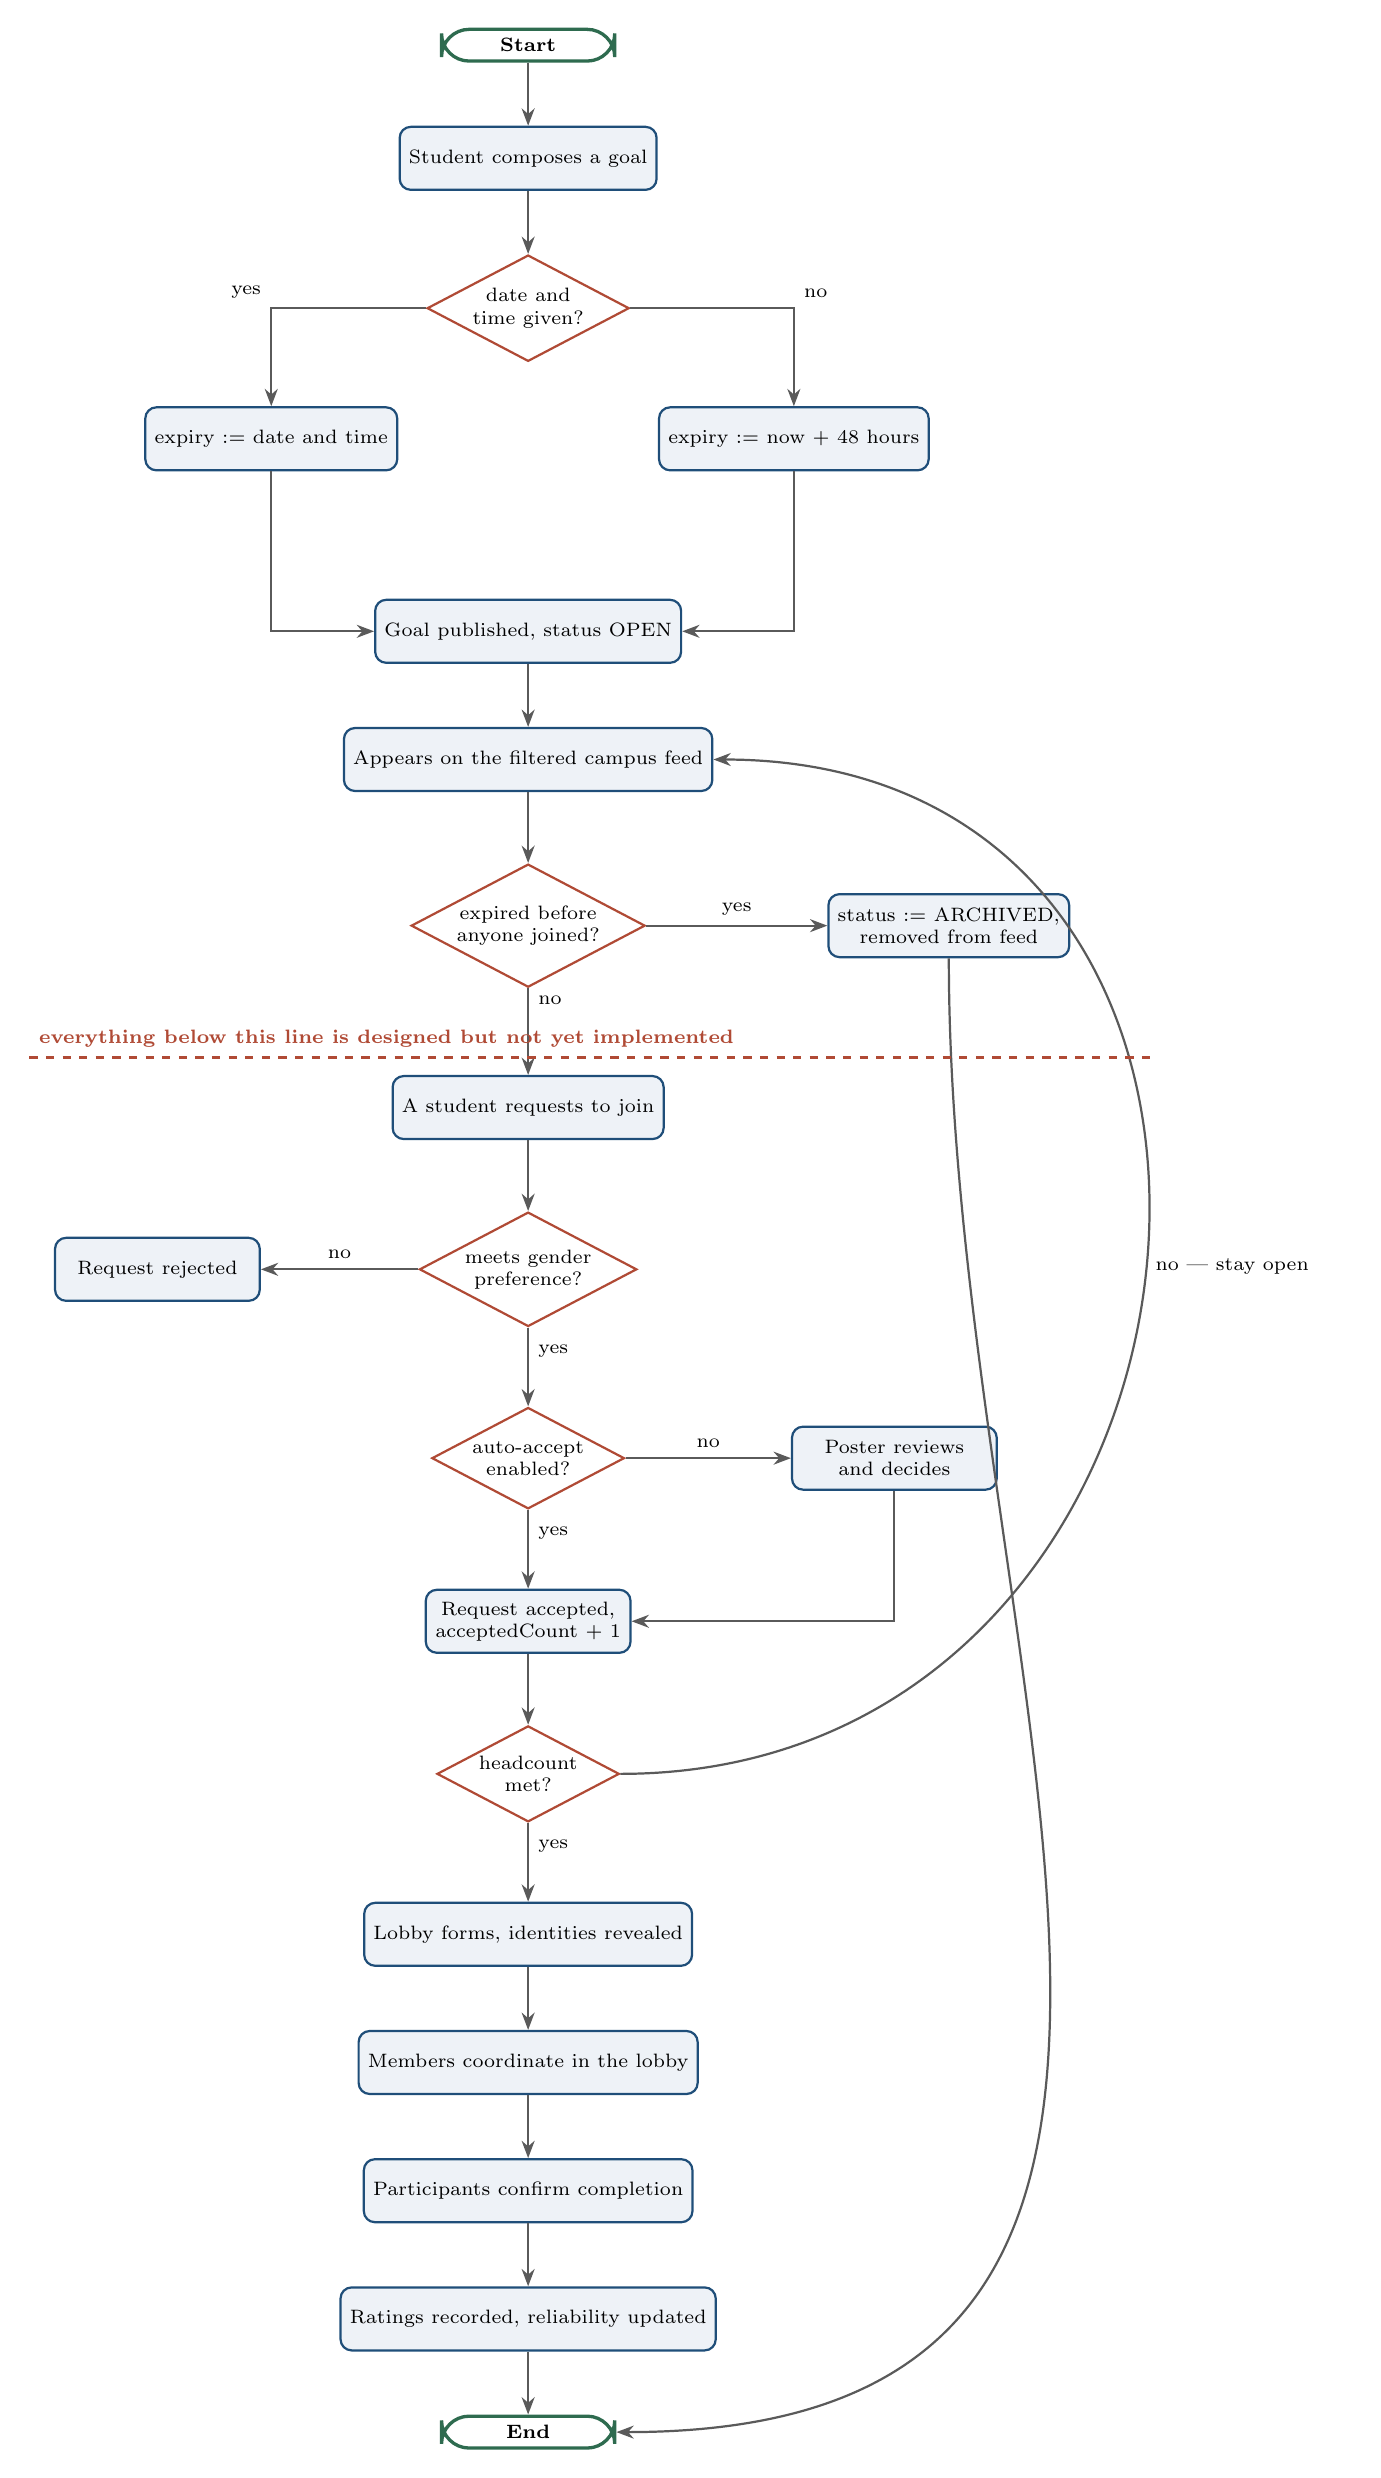
\begin{tikzpicture}[node distance=0.9cm and 1.5cm]

  \node[terminal] (start) {Start};
  \node[act, below=0.8cm of start] (compose) {Student composes a goal};
  \node[decision, below=0.8cm of compose] (dated) {date and\\time given?};
  \node[act, below left=0.9cm and 1.0cm of dated] (setexp1) {expiry := date and time};
  \node[act, below right=0.9cm and 1.0cm of dated] (setexp2) {expiry := now + 48 hours};
  \node[act, below=3.0cm of dated] (open) {Goal published, status OPEN};
  \node[act, below=0.8cm of open] (feed) {Appears on the filtered campus feed};

  \node[decision, below=0.9cm of feed] (expired) {expired before\\anyone joined?};
  \node[act, right=2.3cm of expired] (archive) {status := ARCHIVED,\\removed from feed};

  \node[act, below=1.1cm of expired] (req) {A student requests to join};
  \node[decision, below=0.9cm of req] (elig) {meets gender\\preference?};
  \node[act, left=2.0cm of elig] (rejected) {Request rejected};
  \node[decision, below=1.0cm of elig] (auto) {auto-accept\\enabled?};
  \node[act, right=2.1cm of auto] (poster) {Poster reviews\\and decides};
  \node[act, below=1.0cm of auto] (accept) {Request accepted,\\acceptedCount + 1};
  \node[decision, below=0.9cm of accept] (full) {headcount\\met?};
  \node[act, below=1.0cm of full] (lobby) {Lobby forms, identities revealed};
  \node[act, below=0.8cm of lobby] (chat) {Members coordinate in the lobby};
  \node[act, below=0.8cm of chat] (complete) {Participants confirm completion};
  \node[act, below=0.8cm of complete] (rate) {Ratings recorded, reliability updated};
  \node[terminal, below=0.8cm of rate] (end) {End};

  \draw[flow] (start) -- (compose);
  \draw[flow] (compose) -- (dated);
  \draw[flow] (dated) -| node[above left,font=\scriptsize]{yes} (setexp1);
  \draw[flow] (dated) -| node[above right,font=\scriptsize]{no} (setexp2);
  \draw[flow] (setexp1) |- (open);
  \draw[flow] (setexp2) |- (open);
  \draw[flow] (open) -- (feed);
  \draw[flow] (feed) -- (expired);
  \draw[flow] (expired) -- node[above,font=\scriptsize]{yes} (archive);
  \draw[flow] (expired) -- node[right,font=\scriptsize,pos=0.14]{no} (req);
  \draw[flow] (req) -- (elig);
  \draw[flow] (elig) -- node[above,font=\scriptsize]{no} (rejected);
  \draw[flow] (elig) -- node[right,font=\scriptsize,pos=0.3]{yes} (auto);
  \draw[flow] (auto) -- node[above,font=\scriptsize]{no} (poster);
  \draw[flow] (poster) |- (accept);
  \draw[flow] (auto) -- node[right,font=\scriptsize,pos=0.3]{yes} (accept);
  \draw[flow] (accept) -- (full);
  \draw[flow] (full) -- node[right,font=\scriptsize,pos=0.3]{yes} (lobby);
  \draw[flow] (full.east) to[out=0,in=0,looseness=1.6]
    node[right,font=\scriptsize,pos=0.5]{no — stay open} (feed.east);
  \draw[flow] (lobby) -- (chat);
  \draw[flow] (chat) -- (complete);
  \draw[flow] (complete) -- (rate);
  \draw[flow] (rate) -- (end);
  \draw[flow] (archive.south) to[out=-90,in=0,looseness=1.2] (end.east);

  % Boundary between what runs today and what does not.
  \draw[dashed, very thick, tietaccent]
    ($(req.north west)+(-4.6,0.22)$) -- ($(req.north east)+(6.2,0.22)$);
  \node[anchor=west, font=\scriptsize\bfseries, text=tietaccent]
    at ($(req.north west)+(-4.6,0.46)$)
    {everything below this line is designed but not yet implemented};

\end{tikzpicture}%
}
\caption[Activity diagram: goal lifecycle]{Activity diagram for the goal
lifecycle. Expiry is a first-class path, not an afterthought: a goal whose time
has passed leaves the feed whether or not anybody ever joined it.}
\label{fig:activity}
\end{figure}

\section{System Architecture}

\begin{figure}[htbp]
\centering
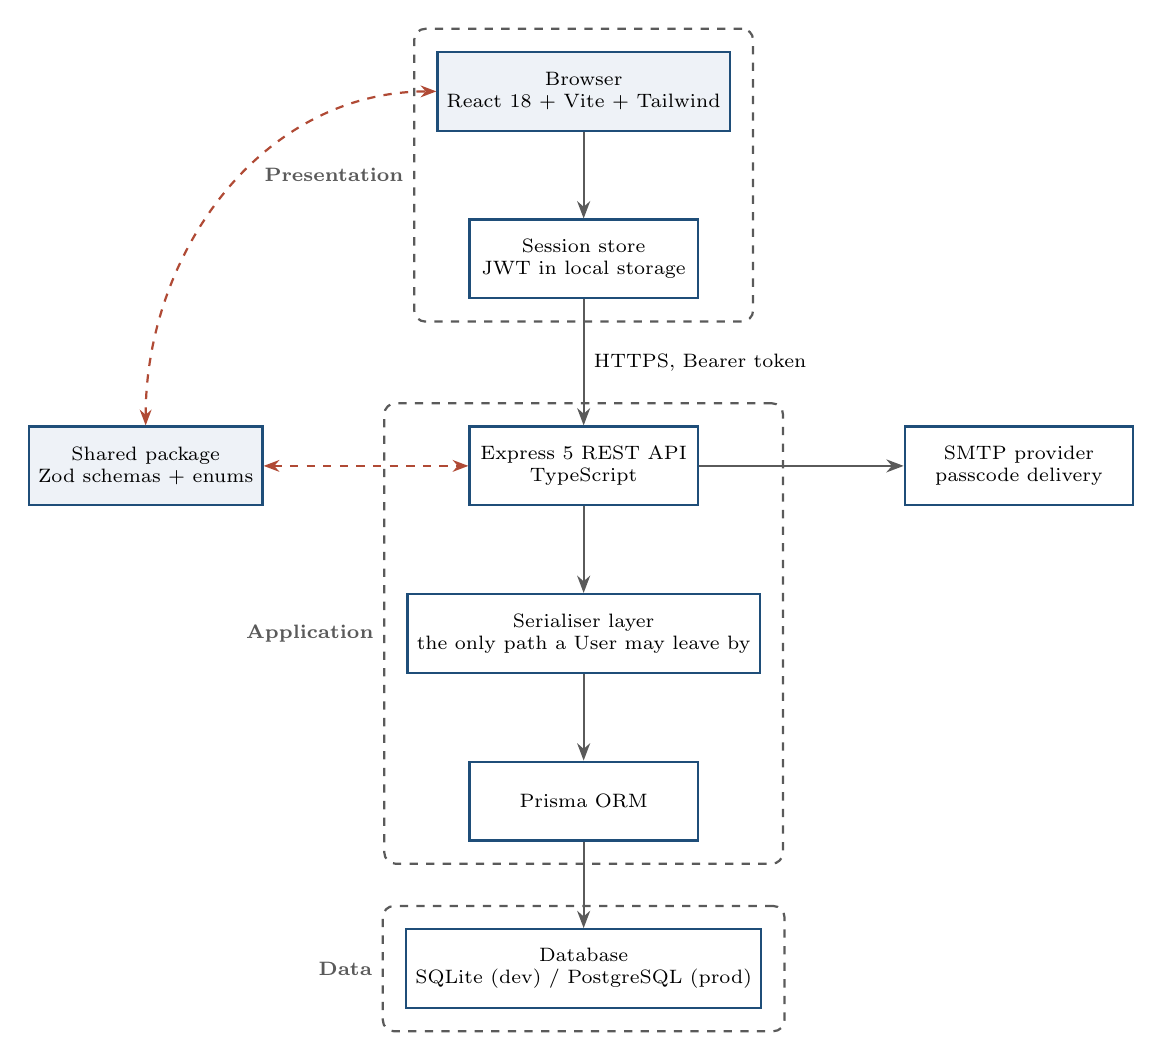
\begin{tikzpicture}[node distance=1.1cm]

  \node[comp, fill=tietlight] (browser) {Browser\\\scriptsize React 18 + Vite + Tailwind};
  \node[comp, below=of browser] (store) {Session store\\\scriptsize JWT in local storage};
  \node[comp, below=1.6cm of store] (api) {Express 5 REST API\\\scriptsize TypeScript};
  \node[comp, below=of api] (serial) {Serialiser layer\\\scriptsize the only path a User may leave by};
  \node[comp, below=of serial] (prisma) {Prisma ORM};
  \node[comp, below=of prisma] (db) {Database\\\scriptsize SQLite (dev) / PostgreSQL (prod)};
  \node[comp, right=2.6cm of api] (mail) {SMTP provider\\\scriptsize passcode delivery};
  \node[comp, left=2.6cm of api, fill=tietlight] (shared) {Shared package\\\scriptsize Zod schemas + enums};

  \draw[flow] (browser) -- (store);
  \draw[flow] (store) -- node[right,font=\scriptsize]{HTTPS, Bearer token} (api);
  \draw[flow] (api) -- (serial);
  \draw[flow] (serial) -- (prisma);
  \draw[flow] (prisma) -- (db);
  \draw[flow] (api) -- (mail);
  \draw[{Stealth[length=2mm]}-{Stealth[length=2mm]}, thick, tietaccent, dashed]
    (shared) -- (api);
  \draw[{Stealth[length=2mm]}-{Stealth[length=2mm]}, thick, tietaccent, dashed]
    (shared.north) to[out=90,in=180] (browser.west);

  \node[draw=tietgrey, dashed, thick, rounded corners, fit=(browser)(store),
        inner sep=8pt, label={[font=\scriptsize\bfseries,text=tietgrey]left:Presentation}] {};
  \node[draw=tietgrey, dashed, thick, rounded corners, fit=(api)(serial)(prisma),
        inner sep=8pt, label={[font=\scriptsize\bfseries,text=tietgrey]left:Application}] {};
  \node[draw=tietgrey, dashed, thick, rounded corners, fit=(db),
        inner sep=8pt, label={[font=\scriptsize\bfseries,text=tietgrey]left:Data}] {};

\end{tikzpicture}
\caption[System architecture]{Three-tier architecture. The shared package is
imported by both the client and the server, which is what guarantees that a form
enforces exactly the rule the API will apply.}
\label{fig:arch}
\end{figure}

%==============================================================================
\chapter{Implementation}
\label{ch:implementation}
%==============================================================================

\section{Technology Stack}

\begin{longtable}{@{}p{3.0cm}p{4.6cm}p{5.4cm}@{}}
\toprule
\textbf{Layer} & \textbf{Chosen} & \textbf{Reason} \\
\midrule
\endhead
Frontend & React 18, Vite, Tailwind CSS v4, React Router 7, Zustand &
Plain JavaScript throughout. Vite gives an instant development server; Zustand
holds only the session, which is the only genuinely global state. \\
\addlinespace
Backend & Node.js, Express 5, TypeScript &
Express 5 forwards rejected promises to the error handler natively, which
removed an entire wrapper the team had written by hand. \\
\addlinespace
Database & Prisma ORM; SQLite in development, PostgreSQL in production &
No database installation on any team member's machine, and one schema file that
runs on both. \\
\addlinespace
Validation & Zod, in a package shared by both sides &
One definition of every rule. \\
\addlinespace
Auth & JWT sessions; scrypt password hashing &
See Section~\ref{sec:decisions}. \\
\addlinespace
Mail & Pluggable transport: console in development, SMTP in production &
Development needs no mail account; production delivers real passcodes. \\
\bottomrule
\end{longtable}

\section{Repository Structure}

The application is an npm workspace with three packages.

\begin{lstlisting}
code/
  frontend/    React client, plain JavaScript
    src/{api,components,pages,store,hooks,lib}
  backend/     Express + Prisma REST API, TypeScript
    prisma/schema.prisma      the executable class diagram
    src/config/               validated environment
    src/lib/                  AppError, password, otp, jwt
    src/middleware/           error handling, requireAuth
    src/serializers/          DTO layer - nothing else returns a User
    src/services/mail/        console and SMTP transports
    src/modules/              one folder per feature
  shared/      enums, constants and Zod schemas used by both sides
\end{lstlisting}

The repository is deliberately mixed-language: a TypeScript API and a JavaScript
client. The shared package is authored in plain JavaScript so the client can
import it directly, and the TypeScript API consumes the identical files.

\section{Implemented API Endpoints}

\begin{longtable}{@{}p{1.6cm}p{5.4cm}p{6.0cm}@{}}
\toprule
\textbf{Method} & \textbf{Path} & \textbf{Purpose} \\
\midrule
\endhead
GET    & \texttt{/api/health}           & Liveness and database check \\
POST   & \texttt{/api/auth/signup}      & Register; sends a passcode \\
POST   & \texttt{/api/auth/verify-otp}  & Confirm the passcode, issue a token \\
POST   & \texttt{/api/auth/resend-otp}  & Reissue a passcode \\
POST   & \texttt{/api/auth/login}       & Authenticate a returning student \\
GET    & \texttt{/api/auth/me}          & Current session \\
GET    & \texttt{/api/users/me}         & Own profile, including private fields \\
PATCH  & \texttt{/api/users/me}         & Update own profile \\
POST   & \texttt{/api/users/me/photo}   & Upload a profile photograph \\
DELETE & \texttt{/api/users/me/photo}   & Remove the photograph \\
GET    & \texttt{/api/users/:id}        & Another student's public profile \\
GET    & \texttt{/api/users/:id/photo}  & Serve a photograph \\
POST   & \texttt{/api/goals}            & Post a goal \\
GET    & \texttt{/api/goals}            & Feed: filtered, cursor-paginated \\
GET    & \texttt{/api/goals/:id}        & One goal \\
DELETE & \texttt{/api/goals/:id}        & Cancel own goal \\
\bottomrule
\end{longtable}

\section{Significant Engineering Decisions}
\label{sec:decisions}

\subsection{Anonymity is enforced in one place, by omission}

The serialiser decides whether a poster's identity is included in a response:

\begin{lstlisting}
const isOwnGoal = goal.posterId === viewer.viewerId;
const identityRevealed =
  !goal.anonymous || isOwnGoal || viewer.viewerIsAcceptedMember === true;

poster: identityRevealed
  ? { isAnonymous: false, ...toPublicUserDTO(goal.poster) }
  : { isAnonymous: true,
      reliabilityScore: goal.poster.reliabilityScore,
      goalsCompleted:   goal.poster.goalsCompleted }
\end{lstlisting}

When a goal is anonymous, the name, identifier and photograph are not included
in the payload at all. A modified client cannot reveal what it was never sent.
This was verified from a second real account: the response contained the
reliability score and nothing else identifying.

\subsection{Profiles cannot be self-promoted}

\texttt{PATCH /api/users/me} is guarded twice against mass assignment. The
validation schema is strict and contains no \texttt{role}, \texttt{isVerified} or
\texttt{reliabilityScore} key, and the service constructs its database write from
an explicit list of permitted fields rather than spreading the request body. A
trust layer is worth nothing if a student can set their own reliability score, so
it is defended in two independent places and asserted by test.

\subsection{Passwords use scrypt from the standard library}

Argon2 and bcrypt both require a native compilation step, and the package manager
now blocks install scripts by default. A dependency that a teammate cannot
install on a fresh clone is a worse outcome than a slightly older key derivation
function. The cost parameters are stored inside each hash, so they can be raised
later without invalidating existing passwords.

\subsection{Authentication endpoints do not disclose who has an account}

A wrong password and an unknown address return an identical response. Requesting
a new passcode returns the same message whether or not the address is
registered. Otherwise either endpoint becomes a way of testing which students
have signed up.

\subsection{The feed is cursor-paginated}

The feed is ordered newest first and new goals arrive continuously. With an
offset, a goal posted while somebody is scrolling shifts every later page and the
reader sees duplicates. A cursor is stable under insertion. Expired goals are
excluded in the query itself, so the feed is correct even before any sweep job
has run.

%==============================================================================
\chapter{Testing and Verification}
\label{ch:testing}
%==============================================================================

\section{Approach}

Testing is automated and runs on every push through continuous integration. The
suite currently contains \textbf{94 tests}, all passing. Integration tests run
against a real database rather than a mocked one, because most of the behaviour
worth testing is the interaction between validation, the service layer and the
schema.

\begin{longtable}{@{}p{4.2cm}p{9.0cm}@{}}
\toprule
\textbf{Kind} & \textbf{What it covers} \\
\midrule
\endhead
Unit &
Passcode generation and hashing, password hashing and comparison, profile
completeness scoring, email templates, date and time conversion. \\
\addlinespace
Integration &
Every endpoint, driven through the HTTP layer against a real database:
registration, verification, login, profile update, photograph upload, goal
creation, the feed and its filters, and cancellation. \\
\addlinespace
Security assertions &
That a non-institute address is rejected; that a passcode cannot be reused or
brute-forced; that an anonymous goal leaks nothing; that a profile update cannot
change role or reliability, asserted against the stored row. \\
\bottomrule
\end{longtable}

\section{Continuous Integration}

Every push runs, in order: formatting check, lint, type check, the full test
suite, and a production build of both applications. A commit that breaks any of
these fails visibly rather than being discovered later.

\section{A Defect Found by Visual Verification}

Not every defect is reachable by an automated test, and it is worth recording one
that was not. Goals posted with a date and time were being stored with no time at
all and displayed as ``Anytime'' on the feed --- for one team member and not the
other. The tests passed throughout, because the value was lost in the browser
before any request was made.

The cause was a single combined date-and-time input. It produces a string with
neither seconds nor a time zone, which one browser's date parser rejects; the
conversion therefore threw inside an event handler, where nothing catches it, and
the field silently never updated. The fix was to split it into separate date and
time fields, parse the parts explicitly rather than relying on the browser's
parser, block submission when only one half is filled in, and display the parsed
result back to the student before posting.

The lesson recorded here is that a silent failure is worse than a loud one. The
implementation now makes this class of error visible at the point it occurs.

%==============================================================================
\chapter{Current Status and Results}
\label{ch:status}
%==============================================================================

\section{What Works Today}

The prototype is a running system, not a mock-up. End to end, a student can:

\begin{enumerate}[leftmargin=*]
  \item Register with a \texttt{@thapar.edu} address --- any other domain is
    rejected at both the client and the server.
  \item Receive a real six-digit passcode in their actual institute inbox,
    delivered over SMTP.
  \item Verify, and be issued a session.
  \item Complete a profile: branch, year of study, gender, interests and a
    photograph.
  \item Post a goal, optionally anonymous, optionally restricted by gender
    preference, optionally auto-accepting.
  \item Browse the campus feed, filter it by category, open a goal and cancel
    their own.
\end{enumerate}

\section{Development Progress}

The project is built in vertical slices. Each step is one feature implemented end
to end --- schema, API, interface and tests --- and is left runnable before the
next begins.

\begin{longtable}{@{}p{1.6cm}p{8.6cm}p{3.0cm}@{}}
\toprule
\textbf{Step} & \textbf{Content} & \textbf{Status} \\
\midrule
\endhead
0 & Repository, tooling, health check, continuous integration & Complete \\
1 & Registration, passcode verification, login, sessions & Complete \\
2 & Profiles: branch, year, gender, interests, photograph & Complete \\
3 & Posting a goal, the public feed, the anonymity serialiser & Complete \\
4 & Requesting to join and poster approval & Next \\
5--12 & Lobbies, chat, notes sharing, trust and safety, ratings, matching,
        metrics, deployment & Planned \\
\bottomrule
\end{longtable}

\section{What Does Not Work Yet}

Stated plainly, because a report that claims more than the software does is worth
less than one that does not: \textbf{a student cannot yet join a goal.} The
request button is deliberately rendered disabled. Everything up to and including
discovery works; the request and approval state machine is the next step, and the
serialiser already accepts the viewer's membership status so that anonymity will
lift for an accepted requester without further change.

\section{Deviations from the Proposal}

Two items in the original proposal were deliberately removed rather than built.

\begin{description}[leftmargin=0.8cm,style=nextline]
  \item[Hostel block and proximity-based matching.]
    Cut as complexity that did not earn its place. With a pilot confined to one
    batch, proximity has almost nothing to discriminate on, while the field would
    have appeared in the profile, the matching logic and the feed filters. Interest,
    branch and past-category scoring are retained for the matching step.

  \item[The choice between MongoDB and PostgreSQL, and between Express and NestJS.]
    The proposal left these open. They are now settled: PostgreSQL through Prisma,
    and Express. A relational schema is the right shape for data that is almost
    entirely relationships, and the join between goals, requests and members is
    the central query of the product.
\end{description}

\section{Known Limitation}

Alias addresses --- a tag after a plus sign, or additional dots in the local part
--- are currently accepted as distinct accounts even though the mail provider
delivers them all to one inbox. A student could therefore hold several verified
accounts and shed a poor reliability score by registering again. This is accepted
deliberately for a pilot of fifteen to twenty people; the remedy, if it is ever
needed, is a canonicalised email column carrying a uniqueness constraint.

%==============================================================================
\chapter{Remaining Work}
%==============================================================================

\begin{longtable}{@{}p{1.5cm}p{7.4cm}p{4.4cm}@{}}
\toprule
\textbf{Step} & \textbf{Work} & \textbf{Delivers} \\
\midrule
\endhead
4 & Request and approval state machine: eligibility checks, capacity, automatic
    acceptance, identity reveal on acceptance & FR-11, FR-12 \\
5 & Lobby formation and membership & FR-13 \\
6 & Real-time lobby chat over web sockets & FR-14 \\
7 & Notes and resource sharing & Proposal \S3.2 \\
8 & Reporting, blocking, moderator review with audit logging & FR-16, FR-17 \\
9 & Ratings, no-show flagging, reliability recalculation & FR-15 \\
10 & Rule-based matching on interest, branch and past categories & Proposal \S3.3 \\
11 & Expiry sweep and fulfilment metrics & FR-9, NFR-4 \\
12 & Deployment & --- \\
\bottomrule
\end{longtable}

%==============================================================================
\chapter{Conclusion}
%==============================================================================

At the prototype stage CampusLink is a working, verified system covering the
first half of its central loop. A student can be admitted to the platform only by
proving they hold an institute email address, can describe themselves, can post
what they want to do, and can discover what everybody else wants to do. Ninety-four
automated tests, a continuous integration pipeline and a clean production build
stand behind that claim.

The design decisions the team is most confident defending are the ones where a
promise to the user is enforced by structure rather than by intention: anonymity
implemented as omission from the response rather than concealment in the
interface, and privilege escalation blocked in two independent places rather
than one. Those are the properties that would survive somebody deliberately
attacking the system, and they were built before the features that depend on
them.

The immediate next step is the request and approval state machine, which turns
the feed from a noticeboard into the product the proposal describes.

\end{document}
